%! Author = Len Washington III
%! Date = 10/29/2023

% Preamble
\documentclass[chapter=7,section=4]{math252homework}
\captionsetup[figure]{labelfont={bf},labelformat={default},name={FIGURE },labelsep=space}
\renewcommand\thefigure{\arabic{chapter}.\arabic{section}.\arabic{problemsi}}

% Document
\begin{document}

In Problems 1--8 use Theorem 7.4.1 to evaluate the given Laplace transform.
\begin{problems}
	\problem \[ \laplace[te^{-10t}] \]
	% TODO: Problem 1
	\setcounter{problemsi}{2}
	\problem \[ \laplace[t\cos(2t)] \]
	% TODO: Problem 3
	\setcounter{problemsi}{5}
	\problem \[ \laplace[t\sinh(3t)] \]
	% TODO: Problem 6
\end{problems}

In Problems 9--14 use the Laplace transform to solve the given initial-value problem. Use the table of Laplace transforms in Appendix C as needed.
\begin{problems}[start=9]
	\problem \[ y' + y = t\sin t,\ivpsep y(0)=0 \]
	% TODO: Problem 9
	\setcounter{problemsi}{11}
	\problem \[ y'' + y = \sin t,\ivpsep y(0)=1,\ivpsep y'(0)=-1 \]
	% TODO: Problem 12
	\problem \[ y'' + 16y = f(t),\ivpsep y(0)=0,\ivpsep y'(0)=1, \mbox{ where }\\f(t) = \left\{ \begin{array}{lr}
		\cos 4t, & 0 \leq t < \pi,\\
		0, & t \geq \pi
	\end{array} \right. \]
	% TODO: Problem 13
\end{problems}

In Problems 19--22 proceed as in Example 3 and find the convolution $f\times g$ of the given functions. After integrating, find the Laplace transform of $f\times g$.
\begin{problems}[start=19]
	\problem \[ f(t) = 4t,\ivpsep g(t) = 3t^{2} \]
	% TODO: Problem 19
	\problem \[ f(t) = t,\ivpsep g(t)=e^{-t} \]
	% TODO: Problem 20
\end{problems}

In Problems 23--34 proceed as in Example 4 and find the Laplace transform of $f\times g$ using Theorem 7.4.2. Do not evaluate the convolution integral before transforming.
\begin{problems}[start=25]
	\problem \[ \laplace[e^{-t}\times e^{t}\cos(t)] \]
	% TODO: Problem 25
	\problem \[ \laplace[e^{2t}\times\sin t] \]
	% TODO: Problem 26
	\problem \[ \laplace[\int_{0}^{t} e^{\tau}d\tau] \]
	% TODO: Problem 27
	\problem \[ \laplace[\int_{0}^{t} \cos(\tau) d\tau] \]
	% TODO: Problem 28
	\setcounter{problemsi}{30}
	\problem \[ \laplace[\int_{0}^{t} e\tau^{t-\tau}d\tau] \]
	% TODO: Problem 31
	\setcounter{problemsi}{32}
	\problem \[ \laplace[\int_{0}^{t} \sin(\tau)d\tau] \]
	% TODO: Problem 33
\end{problems}

In Problems 41--50 use the Laplace transform to solve the given integral equation or integrodifferential equation.
\begin{problems}[start=41]
	\problem \[ f(t) + \int_{0}^{t} (t-\tau)f(\tau)d\tau = t \]
	% TODO: Problem 41
	\setcounter{problemsi}{42}
	\problem \[ f(t) = te^{t} + \int_{0}^{t} \tau f(t-\tau)d\tau \]
	% TODO: Problem 43
	\problem \[ f(t) + 2\int_{0}^{t}f(\tau)\cos(t-\tau)d\tau = 4e^{-t} + \sin t  \]
	% TODO: Problem 44
	\problem \[ f(t) + \int_{0}^{t} f(\tau)d\tau = 1 \]
	% TODO: Problem 45
\end{problems}

In Problems 53--58 use Theorem 7.4.3 to find the Laplace transform of the given periodic function.
\begin{problems}[start=53]
	\problem~\begin{figure}[H]
				 \centering
				 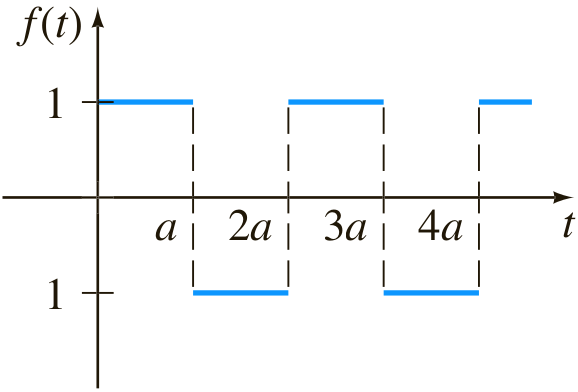
\includegraphics[width=0.5\textwidth]{7.4.53}
				 \caption{Graph for Problem \arabic{problemsi}}
				 \label{fig:meander-function}
	\end{figure}
	% TODO: Problem 53
	\setcounter{problemsi}{54}
	\problem~\begin{figure}[H]
				 \centering
				 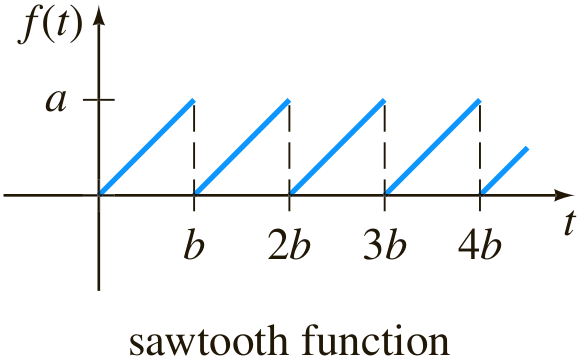
\includegraphics[width=0.5\textwidth]{7.4.55}
				 \caption{Graph for Problem \arabic{problemsi}}
				 \label{fig:sawtooth-function}
	\end{figure}
	% TODO: Problem 55
	\problem~\begin{figure}[H]
				 \centering
				 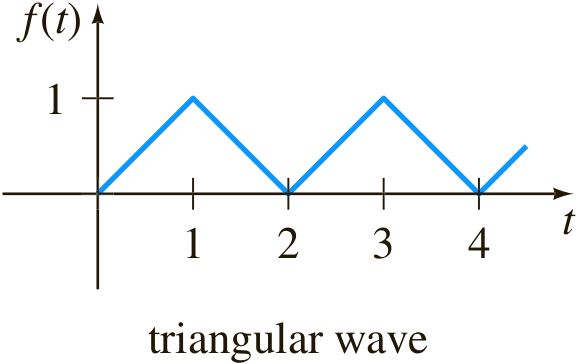
\includegraphics[width=0.5\textwidth]{7.4.56}
				 \caption{Graph for Problem \arabic{problemsi}}
				 \label{fig:triangular-waveS}
	\end{figure}
	% TODO: Problem 56
\end{problems}

\end{document}